\documentclass[1p]{elsarticle_modified}
%\bibliographystyle{elsarticle-num}

%\usepackage[colorlinks]{hyperref}
%\usepackage{abbrmath_seonhwa} %\Abb, \Ascr, \Acal ,\Abf, \Afrak
\usepackage{amsfonts}
\usepackage{amssymb}
\usepackage{amsmath}
\usepackage{amsthm}
\usepackage{scalefnt}
\usepackage{amsbsy}
\usepackage{kotex}
\usepackage{caption}
\usepackage{subfig}
\usepackage{color}
\usepackage{graphicx}
\usepackage{xcolor} %% white, black, red, green, blue, cyan, magenta, yellow
\usepackage{float}
\usepackage{setspace}
\usepackage{hyperref}

\usepackage{tikz}
\usetikzlibrary{arrows}

\usepackage{multirow}
\usepackage{array} % fixed length table
\usepackage{hhline}

%%%%%%%%%%%%%%%%%%%%%
\makeatletter
\renewcommand*\env@matrix[1][\arraystretch]{%
	\edef\arraystretch{#1}%
	\hskip -\arraycolsep
	\let\@ifnextchar\new@ifnextchar
	\array{*\c@MaxMatrixCols c}}
\makeatother %https://tex.stackexchange.com/questions/14071/how-can-i-increase-the-line-spacing-in-a-matrix
%%%%%%%%%%%%%%%

\usepackage[normalem]{ulem}

\newcommand{\msout}[1]{\ifmmode\text{\sout{\ensuremath{#1}}}\else\sout{#1}\fi}
%SOURCE: \msout is \stkout macro in https://tex.stackexchange.com/questions/20609/strikeout-in-math-mode

\newcommand{\cancel}[1]{
	\ifmmode
	{\color{red}\msout{#1}}
	\else
	{\color{red}\sout{#1}}
	\fi
}

\newcommand{\add}[1]{
	{\color{blue}\uwave{#1}}
}

\newcommand{\replace}[2]{
	\ifmmode
	{\color{red}\msout{#1}}{\color{blue}\uwave{#2}}
	\else
	{\color{red}\sout{#1}}{\color{blue}\uwave{#2}}
	\fi
}

\newcommand{\Sol}{\mathcal{S}} %segment
\newcommand{\D}{D} %diagram
\newcommand{\A}{\mathcal{A}} %arc


%%%%%%%%%%%%%%%%%%%%%%%%%%%%%5 test

\def\sl{\operatorname{\textup{SL}}(2,\Cbb)}
\def\psl{\operatorname{\textup{PSL}}(2,\Cbb)}
\def\quan{\mkern 1mu \triangleright \mkern 1mu}

\theoremstyle{definition}
\newtheorem{thm}{Theorem}[section]
\newtheorem{prop}[thm]{Proposition}
\newtheorem{lem}[thm]{Lemma}
\newtheorem{ques}[thm]{Question}
\newtheorem{cor}[thm]{Corollary}
\newtheorem{defn}[thm]{Definition}
\newtheorem{exam}[thm]{Example}
\newtheorem{rmk}[thm]{Remark}
\newtheorem{alg}[thm]{Algorithm}

\newcommand{\I}{\sqrt{-1}}
\begin{document}

%\begin{frontmatter}
%
%\title{Boundary parabolic representations of knots up to 8 crossings}
%
%%% Group authors per affiliation:
%\author{Yunhi Cho} 
%\address{Department of Mathematics, University of Seoul, Seoul, Korea}
%\ead{yhcho@uos.ac.kr}
%
%
%\author{Seonhwa Kim} %\fnref{s_kim}}
%\address{Center for Geometry and Physics, Institute for Basic Science, Pohang, 37673, Korea}
%\ead{ryeona17@ibs.re.kr}
%
%\author{Hyuk Kim}
%\address{Department of Mathematical Sciences, Seoul National University, Seoul 08826, Korea}
%\ead{hyukkim@snu.ac.kr}
%
%\author{Seokbeom Yoon}
%\address{Department of Mathematical Sciences, Seoul National University, Seoul, 08826,  Korea}
%\ead{sbyoon15@snu.ac.kr}
%
%\begin{abstract}
%We find all boundary parabolic representation of knots up to 8 crossings.
%
%\end{abstract}
%\begin{keyword}
%    \MSC[2010] 57M25 
%\end{keyword}
%
%\end{frontmatter}

%\linenumbers
%\tableofcontents
%
\newcommand\colored[1]{\textcolor{white}{\rule[-0.35ex]{0.8em}{1.4ex}}\kern-0.8em\color{red} #1}%
%\newcommand\colored[1]{\textcolor{white}{ #1}\kern-2.17ex	\textcolor{white}{ #1}\kern-1.81ex	\textcolor{white}{ #1}\kern-2.15ex\color{red}#1	}

{\Large $\underline{12a_{1186}~(K12a_{1186})}$}

\setlength{\tabcolsep}{10pt}
\renewcommand{\arraystretch}{1.6}
\vspace{1cm}\begin{tabular}{m{100pt}>{\centering\arraybackslash}m{274pt}}
\multirow{5}{120pt}{
	\centering
	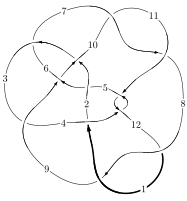
\includegraphics[width=112pt]{../../../GIT/diagram.site/Diagrams/png/1987_12a_1186.png}\\
\ \ \ A knot diagram\footnotemark}&
\allowdisplaybreaks
\textbf{Linearized knot diagam} \\
\cline{2-2}
 &
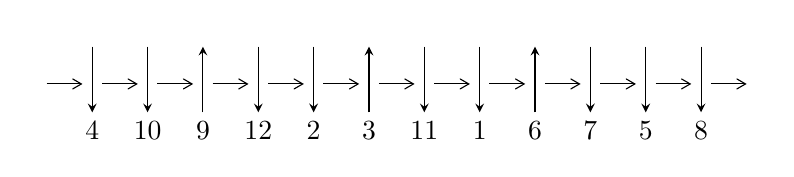
\begin{tikzpicture}[x=20pt, y=17pt]
	% nodes
	\node (C0) at (0, 0) {};
	\node (C1) at (1, 0) {};
	\node (C1U) at (1, +1) {};
	\node (C1D) at (1, -1) {4};

	\node (C2) at (2, 0) {};
	\node (C2U) at (2, +1) {};
	\node (C2D) at (2, -1) {10};

	\node (C3) at (3, 0) {};
	\node (C3U) at (3, +1) {};
	\node (C3D) at (3, -1) {9};

	\node (C4) at (4, 0) {};
	\node (C4U) at (4, +1) {};
	\node (C4D) at (4, -1) {12};

	\node (C5) at (5, 0) {};
	\node (C5U) at (5, +1) {};
	\node (C5D) at (5, -1) {2};

	\node (C6) at (6, 0) {};
	\node (C6U) at (6, +1) {};
	\node (C6D) at (6, -1) {3};

	\node (C7) at (7, 0) {};
	\node (C7U) at (7, +1) {};
	\node (C7D) at (7, -1) {11};

	\node (C8) at (8, 0) {};
	\node (C8U) at (8, +1) {};
	\node (C8D) at (8, -1) {1};

	\node (C9) at (9, 0) {};
	\node (C9U) at (9, +1) {};
	\node (C9D) at (9, -1) {6};

	\node (C10) at (10, 0) {};
	\node (C10U) at (10, +1) {};
	\node (C10D) at (10, -1) {7};

	\node (C11) at (11, 0) {};
	\node (C11U) at (11, +1) {};
	\node (C11D) at (11, -1) {5};

	\node (C12) at (12, 0) {};
	\node (C12U) at (12, +1) {};
	\node (C12D) at (12, -1) {8};
	\node (C13) at (13, 0) {};

	% arrows
	\draw[->,>={angle 60}]
	(C0) edge (C1) (C1) edge (C2) (C2) edge (C3) (C3) edge (C4) (C4) edge (C5) (C5) edge (C6) (C6) edge (C7) (C7) edge (C8) (C8) edge (C9) (C9) edge (C10) (C10) edge (C11) (C11) edge (C12) (C12) edge (C13) ;	\draw[->,>=stealth]
	(C1U) edge (C1D) (C2U) edge (C2D) (C3D) edge (C3U) (C4U) edge (C4D) (C5U) edge (C5D) (C6D) edge (C6U) (C7U) edge (C7D) (C8U) edge (C8D) (C9D) edge (C9U) (C10U) edge (C10D) (C11U) edge (C11D) (C12U) edge (C12D) ;
	\end{tikzpicture} \\
\hhline{~~} \\& 
\textbf{Solving Sequence} \\ \cline{2-2} 
 &
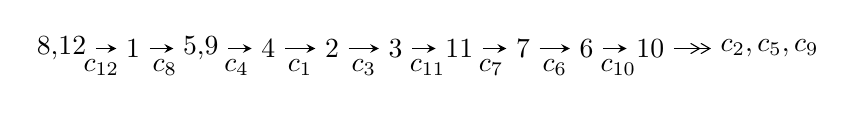
\begin{tikzpicture}[x=23pt, y=7pt]
	% node
	\node (A0) at (-1/8, 0) {8,12};
	\node (A1) at (1, 0) {1};
	\node (A2) at (33/16, 0) {5,9};
	\node (A3) at (25/8, 0) {4};
	\node (A4) at (33/8, 0) {2};
	\node (A5) at (41/8, 0) {3};
	\node (A6) at (49/8, 0) {11};
	\node (A7) at (57/8, 0) {7};
	\node (A8) at (65/8, 0) {6};
	\node (A9) at (73/8, 0) {10};
	\node (C1) at (1/2, -1) {$c_{12}$};
	\node (C2) at (3/2, -1) {$c_{8}$};
	\node (C3) at (21/8, -1) {$c_{4}$};
	\node (C4) at (29/8, -1) {$c_{1}$};
	\node (C5) at (37/8, -1) {$c_{3}$};
	\node (C6) at (45/8, -1) {$c_{11}$};
	\node (C7) at (53/8, -1) {$c_{7}$};
	\node (C8) at (61/8, -1) {$c_{6}$};
	\node (C9) at (69/8, -1) {$c_{10}$};
	\node (A10) at (11, 0) {$c_{2},c_{5},c_{9}$};

	% edge
	\draw[->,>=stealth]	
	(A0) edge (A1) (A1) edge (A2) (A2) edge (A3) (A3) edge (A4) (A4) edge (A5) (A5) edge (A6) (A6) edge (A7) (A7) edge (A8) (A8) edge (A9) ;
	\draw[->>,>={angle 60}]	
	(A9) edge (A10);
\end{tikzpicture} \\ 

\end{tabular} \\

\footnotetext{
The image of knot diagram is generated by the software ``\textbf{Draw programme}" developed by Andrew Bartholomew(\url{http://www.layer8.co.uk/maths/draw/index.htm\#Running-draw}), where we modified some parts for our purpose(\url{https://github.com/CATsTAILs/LinksPainter}).
}\phantom \\ \newline 
\centering \textbf{Ideals for irreducible components\footnotemark of $X_{\text{par}}$} 
 
\begin{align*}
I^u_{1}&=\langle 
-4.29362\times10^{974} u^{160}+9.03975\times10^{975} u^{159}+\cdots+2.56768\times10^{977} b-5.48790\times10^{979},\\
\phantom{I^u_{1}}&\phantom{= \langle  }2.14000\times10^{981} u^{160}+8.49665\times10^{979} u^{159}+\cdots+7.75053\times10^{982} a+1.27842\times10^{985},\\
\phantom{I^u_{1}}&\phantom{= \langle  }u^{161}+u^{160}+\cdots+24936 u+6037\rangle \\
I^u_{2}&=\langle 
8.82947\times10^{39} u^{38}-3.03134\times10^{39} u^{37}+\cdots+1.76750\times10^{39} b-1.68233\times10^{39},\\
\phantom{I^u_{2}}&\phantom{= \langle  }6.00426\times10^{41} u^{38}-8.14543\times10^{40} u^{37}+\cdots+4.41875\times10^{40} a+1.01665\times10^{42},\;u^{39}-11 u^{37}+\cdots+3 u-1\rangle \\
\\
\end{align*}
\raggedright * 2 irreducible components of $\dim_{\mathbb{C}}=0$, with total 200 representations.\\
\footnotetext{All coefficients of polynomials are rational numbers. But the coefficients are sometimes approximated in decimal forms when there is not enough margin.}
\newpage
\renewcommand{\arraystretch}{1}
\centering \section*{I. $I^u_{1}= \langle -4.29\times10^{974} u^{160}+9.04\times10^{975} u^{159}+\cdots+2.57\times10^{977} b-5.49\times10^{979},\;2.14\times10^{981} u^{160}+8.50\times10^{979} u^{159}+\cdots+7.75\times10^{982} a+1.28\times10^{985},\;u^{161}+u^{160}+\cdots+24936 u+6037 \rangle$}
\flushleft \textbf{(i) Arc colorings}\\
\begin{tabular}{m{7pt} m{180pt} m{7pt} m{180pt} }
\flushright $a_{8}=$&$\begin{pmatrix}0\\u\end{pmatrix}$ \\
\flushright $a_{12}=$&$\begin{pmatrix}1\\0\end{pmatrix}$ \\
\flushright $a_{1}=$&$\begin{pmatrix}1\\u^2\end{pmatrix}$ \\
\flushright $a_{5}=$&$\begin{pmatrix}-0.0276110 u^{160}-0.00109627 u^{159}+\cdots-596.130 u-164.946\\0.00167218 u^{160}-0.0352059 u^{159}+\cdots+881.794 u+213.730\end{pmatrix}$ \\
\flushright $a_{9}=$&$\begin{pmatrix}- u\\- u^3+u\end{pmatrix}$ \\
\flushright $a_{4}=$&$\begin{pmatrix}-0.0259389 u^{160}-0.0363022 u^{159}+\cdots+285.664 u+48.7846\\0.00167218 u^{160}-0.0352059 u^{159}+\cdots+881.794 u+213.730\end{pmatrix}$ \\
\flushright $a_{2}=$&$\begin{pmatrix}0.0140242 u^{160}+0.0992901 u^{159}+\cdots-2567.63 u-568.860\\0.0512106 u^{160}+0.0914353 u^{159}+\cdots-1358.16 u-259.711\end{pmatrix}$ \\
\flushright $a_{3}=$&$\begin{pmatrix}-0.0283411 u^{160}+0.00279385 u^{159}+\cdots-716.842 u-195.452\\0.00124565 u^{160}-0.0347879 u^{159}+\cdots+864.002 u+207.442\end{pmatrix}$ \\
\flushright $a_{11}=$&$\begin{pmatrix}0.0511473 u^{160}+0.0914235 u^{159}+\cdots-1305.75 u-241.050\\-0.0126687 u^{160}+0.0104702 u^{159}+\cdots-455.455 u-123.126\end{pmatrix}$ \\
\flushright $a_{7}=$&$\begin{pmatrix}0.0636829 u^{160}+0.0996925 u^{159}+\cdots-1408.75 u-255.065\\0.00974077 u^{160}+0.0620108 u^{159}+\cdots-1360.10 u-317.976\end{pmatrix}$ \\
\flushright $a_{6}=$&$\begin{pmatrix}0.0711499 u^{160}+0.0878869 u^{159}+\cdots-1083.95 u-147.955\\0.0378081 u^{160}+0.0759707 u^{159}+\cdots-1106.45 u-204.614\end{pmatrix}$ \\
\flushright $a_{10}=$&$\begin{pmatrix}0.665656 u^{160}+1.37405 u^{159}+\cdots-21354.7 u-4205.34\\-0.0352658 u^{160}-0.0888632 u^{159}+\cdots+1676.79 u+350.164\end{pmatrix}$\\&\end{tabular}
\flushleft \textbf{(ii) Obstruction class $= -1$}\\~\\
\flushleft \textbf{(iii) Cusp Shapes $= -0.338853 u^{160}-0.432348 u^{159}+\cdots+7021.47 u+747.654$}\\~\\
\newpage\renewcommand{\arraystretch}{1}
\flushleft \textbf{(iv) u-Polynomials at the component}\newline \\
\begin{tabular}{m{50pt}|m{274pt}}
Crossings & \hspace{64pt}u-Polynomials at each crossing \\
\hline $$\begin{aligned}c_{1}\end{aligned}$$&$\begin{aligned}
&5(5 u^{161}+14 u^{160}+\cdots+298224 u-35381)
\end{aligned}$\\
\hline $$\begin{aligned}c_{2}\end{aligned}$$&$\begin{aligned}
&u^{161}-9 u^{160}+\cdots-548262 u+99355
\end{aligned}$\\
\hline $$\begin{aligned}c_{3}\end{aligned}$$&$\begin{aligned}
&u^{161}-7 u^{160}+\cdots+4011301212363 u+841089013283
\end{aligned}$\\
\hline $$\begin{aligned}c_{4},c_{11}\end{aligned}$$&$\begin{aligned}
&u^{161}+45 u^{159}+\cdots+4938 u+811
\end{aligned}$\\
\hline $$\begin{aligned}c_{5}\end{aligned}$$&$\begin{aligned}
&u^{161}-2 u^{160}+\cdots+765004288 u+512157412
\end{aligned}$\\
\hline $$\begin{aligned}c_{6}\end{aligned}$$&$\begin{aligned}
&u^{161}-9 u^{160}+\cdots-454022 u-31165
\end{aligned}$\\
\hline $$\begin{aligned}c_{7},c_{10}\end{aligned}$$&$\begin{aligned}
&5(5 u^{161}+13 u^{160}+\cdots-906128 u-1823792)
\end{aligned}$\\
\hline $$\begin{aligned}c_{8},c_{12}\end{aligned}$$&$\begin{aligned}
&u^{161}- u^{160}+\cdots+24936 u-6037
\end{aligned}$\\
\hline $$\begin{aligned}c_{9}\end{aligned}$$&$\begin{aligned}
&5(5 u^{161}-2 u^{160}+\cdots-51 u-1)
\end{aligned}$\\
\hline
\end{tabular}\\~\\
\newpage\renewcommand{\arraystretch}{1}
\flushleft \textbf{(v) Riley Polynomials at the component}\newline \\
\begin{tabular}{m{50pt}|m{274pt}}
Crossings & \hspace{64pt}Riley Polynomials at each crossing \\
\hline $$\begin{aligned}c_{1}\end{aligned}$$&$\begin{aligned}
&25(25 y^{161}-1686 y^{160}+\cdots+4.37080\times10^{11} y-1.25182\times10^{9})
\end{aligned}$\\
\hline $$\begin{aligned}c_{2}\end{aligned}$$&$\begin{aligned}
&y^{161}-85 y^{160}+\cdots+456455767864 y-9871416025
\end{aligned}$\\
\hline $$\begin{aligned}c_{3}\end{aligned}$$&$\begin{aligned}
&y^{161}+49 y^{160}+\cdots-3.51\times10^{25} y-7.07\times10^{23}
\end{aligned}$\\
\hline $$\begin{aligned}c_{4},c_{11}\end{aligned}$$&$\begin{aligned}
&y^{161}+90 y^{160}+\cdots+12246418 y-657721
\end{aligned}$\\
\hline $$\begin{aligned}c_{5}\end{aligned}$$&$\begin{aligned}
&y^{161}-36 y^{160}+\cdots-6.33\times10^{18} y-2.62\times10^{17}
\end{aligned}$\\
\hline $$\begin{aligned}c_{6}\end{aligned}$$&$\begin{aligned}
&y^{161}+61 y^{160}+\cdots+157597174614 y-971257225
\end{aligned}$\\
\hline $$\begin{aligned}c_{7},c_{10}\end{aligned}$$&$\begin{aligned}
&25\\
&\cdot(25 y^{161}-2849 y^{160}+\cdots-219322678065152 y-3326217259264)
\end{aligned}$\\
\hline $$\begin{aligned}c_{8},c_{12}\end{aligned}$$&$\begin{aligned}
&y^{161}-105 y^{160}+\cdots+3354234814 y-36445369
\end{aligned}$\\
\hline $$\begin{aligned}c_{9}\end{aligned}$$&$\begin{aligned}
&25(25 y^{161}+1126 y^{160}+\cdots+1967 y-1)
\end{aligned}$\\
\hline
\end{tabular}\\~\\
\newpage\flushleft \textbf{(vi) Complex Volumes and Cusp Shapes}
$$\begin{array}{c|c|c}  
\text{Solutions to }I^u_{1}& \I (\text{vol} + \sqrt{-1}CS) & \text{Cusp shape}\\
 \hline 
\begin{aligned}
u &= \phantom{-}0.997231 + 0.047117 I \\
a &= -0.43191 - 1.44048 I \\
b &= -0.10014 + 1.49479 I\end{aligned}
 & -1.88652 - 1.20331 I & \phantom{-0.000000 } 0 \\ \hline\begin{aligned}
u &= \phantom{-}0.997231 - 0.047117 I \\
a &= -0.43191 + 1.44048 I \\
b &= -0.10014 - 1.49479 I\end{aligned}
 & -1.88652 + 1.20331 I & \phantom{-0.000000 } 0 \\ \hline\begin{aligned}
u &= \phantom{-}1.001590 + 0.013656 I \\
a &= \phantom{-}4.17228 + 0.26887 I \\
b &= \phantom{-}0.131236 - 0.863602 I\end{aligned}
 & -3.63160 - 0.05409 I & \phantom{-0.000000 } 0 \\ \hline\begin{aligned}
u &= \phantom{-}1.001590 - 0.013656 I \\
a &= \phantom{-}4.17228 - 0.26887 I \\
b &= \phantom{-}0.131236 + 0.863602 I\end{aligned}
 & -3.63160 + 0.05409 I & \phantom{-0.000000 } 0 \\ \hline\begin{aligned}
u &= \phantom{-}0.469079 + 0.869391 I \\
a &= \phantom{-}0.793271 - 0.991446 I \\
b &= -0.603780 + 0.420923 I\end{aligned}
 & -5.56060 - 0.85512 I & \phantom{-0.000000 } 0 \\ \hline\begin{aligned}
u &= \phantom{-}0.469079 - 0.869391 I \\
a &= \phantom{-}0.793271 + 0.991446 I \\
b &= -0.603780 - 0.420923 I\end{aligned}
 & -5.56060 + 0.85512 I & \phantom{-0.000000 } 0 \\ \hline\begin{aligned}
u &= -1.019120 + 0.053244 I \\
a &= -0.106597 - 0.984322 I \\
b &= -0.08565 + 2.19234 I\end{aligned}
 & -2.73668 + 6.02897 I & \phantom{-0.000000 } 0 \\ \hline\begin{aligned}
u &= -1.019120 - 0.053244 I \\
a &= -0.106597 + 0.984322 I \\
b &= -0.08565 - 2.19234 I\end{aligned}
 & -2.73668 - 6.02897 I & \phantom{-0.000000 } 0 \\ \hline\begin{aligned}
u &= -0.879021 + 0.412006 I \\
a &= \phantom{-}1.05605 + 1.06424 I \\
b &= \phantom{-}0.279868 - 0.990779 I\end{aligned}
 & \phantom{-}1.84415 + 2.12053 I & \phantom{-0.000000 } 0 \\ \hline\begin{aligned}
u &= -0.879021 - 0.412006 I \\
a &= \phantom{-}1.05605 - 1.06424 I \\
b &= \phantom{-}0.279868 + 0.990779 I\end{aligned}
 & \phantom{-}1.84415 - 2.12053 I & \phantom{-0.000000 } 0\\
 \hline 
 \end{array}$$\newpage$$\begin{array}{c|c|c}  
\text{Solutions to }I^u_{1}& \I (\text{vol} + \sqrt{-1}CS) & \text{Cusp shape}\\
 \hline 
\begin{aligned}
u &= \phantom{-}0.924911 + 0.273015 I \\
a &= -0.392924 + 0.428602 I \\
b &= \phantom{-}0.40296 - 1.66723 I\end{aligned}
 & -0.86418 - 3.14112 I & \phantom{-0.000000 } 0 \\ \hline\begin{aligned}
u &= \phantom{-}0.924911 - 0.273015 I \\
a &= -0.392924 - 0.428602 I \\
b &= \phantom{-}0.40296 + 1.66723 I\end{aligned}
 & -0.86418 + 3.14112 I & \phantom{-0.000000 } 0 \\ \hline\begin{aligned}
u &= \phantom{-}0.205271 + 1.020660 I \\
a &= -0.38916 + 1.69345 I \\
b &= \phantom{-}0.545906 - 0.623479 I\end{aligned}
 & -4.32822 + 0.22652 I & \phantom{-0.000000 } 0 \\ \hline\begin{aligned}
u &= \phantom{-}0.205271 - 1.020660 I \\
a &= -0.38916 - 1.69345 I \\
b &= \phantom{-}0.545906 + 0.623479 I\end{aligned}
 & -4.32822 - 0.22652 I & \phantom{-0.000000 } 0 \\ \hline\begin{aligned}
u &= \phantom{-}0.234051 + 0.919743 I \\
a &= -0.41837 - 1.46533 I \\
b &= \phantom{-}0.504875 + 1.181830 I\end{aligned}
 & -1.05075 - 5.36609 I & \phantom{-0.000000 } 0 \\ \hline\begin{aligned}
u &= \phantom{-}0.234051 - 0.919743 I \\
a &= -0.41837 + 1.46533 I \\
b &= \phantom{-}0.504875 - 1.181830 I\end{aligned}
 & -1.05075 + 5.36609 I & \phantom{-0.000000 } 0 \\ \hline\begin{aligned}
u &= \phantom{-}0.083853 + 0.943879 I \\
a &= -0.08194 - 1.69278 I \\
b &= -0.338894 + 1.231970 I\end{aligned}
 & \phantom{-}2.03563 + 8.47449 I & \phantom{-0.000000 } 0 \\ \hline\begin{aligned}
u &= \phantom{-}0.083853 - 0.943879 I \\
a &= -0.08194 + 1.69278 I \\
b &= -0.338894 - 1.231970 I\end{aligned}
 & \phantom{-}2.03563 - 8.47449 I & \phantom{-0.000000 } 0 \\ \hline\begin{aligned}
u &= -0.450880 + 0.828705 I \\
a &= \phantom{-}0.374284 + 1.317450 I \\
b &= \phantom{-}0.121510 - 1.181440 I\end{aligned}
 & \phantom{-}2.90186 + 2.53799 I & \phantom{-0.000000 } 0 \\ \hline\begin{aligned}
u &= -0.450880 - 0.828705 I \\
a &= \phantom{-}0.374284 - 1.317450 I \\
b &= \phantom{-}0.121510 + 1.181440 I\end{aligned}
 & \phantom{-}2.90186 - 2.53799 I & \phantom{-0.000000 } 0\\
 \hline 
 \end{array}$$\newpage$$\begin{array}{c|c|c}  
\text{Solutions to }I^u_{1}& \I (\text{vol} + \sqrt{-1}CS) & \text{Cusp shape}\\
 \hline 
\begin{aligned}
u &= \phantom{-}0.929111 + 0.163151 I \\
a &= \phantom{-}0.379863 - 0.077376 I \\
b &= \phantom{-}0.921115 - 0.244664 I\end{aligned}
 & -0.980980 - 0.322040 I & \phantom{-0.000000 } 0 \\ \hline\begin{aligned}
u &= \phantom{-}0.929111 - 0.163151 I \\
a &= \phantom{-}0.379863 + 0.077376 I \\
b &= \phantom{-}0.921115 + 0.244664 I\end{aligned}
 & -0.980980 + 0.322040 I & \phantom{-0.000000 } 0 \\ \hline\begin{aligned}
u &= -0.474653 + 0.805520 I \\
a &= \phantom{-}0.86515 + 1.33187 I \\
b &= -0.518764 - 0.304689 I\end{aligned}
 & -6.19510 + 9.33654 I & \phantom{-0.000000 } 0 \\ \hline\begin{aligned}
u &= -0.474653 - 0.805520 I \\
a &= \phantom{-}0.86515 - 1.33187 I \\
b &= -0.518764 + 0.304689 I\end{aligned}
 & -6.19510 - 9.33654 I & \phantom{-0.000000 } 0 \\ \hline\begin{aligned}
u &= \phantom{-}1.025840 + 0.297656 I \\
a &= \phantom{-}0.943361 + 0.420612 I \\
b &= -0.304974 + 0.689289 I\end{aligned}
 & -3.58960 + 1.06942 I & \phantom{-0.000000 } 0 \\ \hline\begin{aligned}
u &= \phantom{-}1.025840 - 0.297656 I \\
a &= \phantom{-}0.943361 - 0.420612 I \\
b &= -0.304974 - 0.689289 I\end{aligned}
 & -3.58960 - 1.06942 I & \phantom{-0.000000 } 0 \\ \hline\begin{aligned}
u &= -0.832999 + 0.417115 I \\
a &= -1.21518 - 2.35938 I \\
b &= -0.291421 + 0.859200 I\end{aligned}
 & -3.08080 + 1.50448 I & \phantom{-0.000000 } 0 \\ \hline\begin{aligned}
u &= -0.832999 - 0.417115 I \\
a &= -1.21518 + 2.35938 I \\
b &= -0.291421 - 0.859200 I\end{aligned}
 & -3.08080 - 1.50448 I & \phantom{-0.000000 } 0 \\ \hline\begin{aligned}
u &= \phantom{-}1.071430 + 0.010458 I \\
a &= -0.912189 - 0.061666 I \\
b &= -0.398832 - 1.016720 I\end{aligned}
 & -2.30151 - 0.79773 I & \phantom{-0.000000 } 0 \\ \hline\begin{aligned}
u &= \phantom{-}1.071430 - 0.010458 I \\
a &= -0.912189 + 0.061666 I \\
b &= -0.398832 + 1.016720 I\end{aligned}
 & -2.30151 + 0.79773 I & \phantom{-0.000000 } 0\\
 \hline 
 \end{array}$$\newpage$$\begin{array}{c|c|c}  
\text{Solutions to }I^u_{1}& \I (\text{vol} + \sqrt{-1}CS) & \text{Cusp shape}\\
 \hline 
\begin{aligned}
u &= -1.071220 + 0.030154 I \\
a &= -1.13924 - 1.19995 I \\
b &= -0.732485 + 1.068550 I\end{aligned}
 & -6.46533 + 1.37125 I & \phantom{-0.000000 } 0 \\ \hline\begin{aligned}
u &= -1.071220 - 0.030154 I \\
a &= -1.13924 + 1.19995 I \\
b &= -0.732485 - 1.068550 I\end{aligned}
 & -6.46533 - 1.37125 I & \phantom{-0.000000 } 0 \\ \hline\begin{aligned}
u &= -1.024840 + 0.331353 I \\
a &= -0.424494 + 0.514772 I \\
b &= -0.206787 - 0.544013 I\end{aligned}
 & -1.51905 + 4.34421 I & \phantom{-0.000000 } 0 \\ \hline\begin{aligned}
u &= -1.024840 - 0.331353 I \\
a &= -0.424494 - 0.514772 I \\
b &= -0.206787 + 0.544013 I\end{aligned}
 & -1.51905 - 4.34421 I & \phantom{-0.000000 } 0 \\ \hline\begin{aligned}
u &= \phantom{-}0.513031 + 0.967666 I \\
a &= \phantom{-}0.868286 - 0.887208 I \\
b &= -0.253811 + 1.019720 I\end{aligned}
 & -0.761914 + 0.765531 I & \phantom{-0.000000 } 0 \\ \hline\begin{aligned}
u &= \phantom{-}0.513031 - 0.967666 I \\
a &= \phantom{-}0.868286 + 0.887208 I \\
b &= -0.253811 - 1.019720 I\end{aligned}
 & -0.761914 - 0.765531 I & \phantom{-0.000000 } 0 \\ \hline\begin{aligned}
u &= \phantom{-}0.535901 + 0.972225 I \\
a &= -0.581412 + 0.867669 I \\
b &= \phantom{-}0.620190 - 1.083680 I\end{aligned}
 & -0.71369 + 6.13552 I & \phantom{-0.000000 } 0 \\ \hline\begin{aligned}
u &= \phantom{-}0.535901 - 0.972225 I \\
a &= -0.581412 - 0.867669 I \\
b &= \phantom{-}0.620190 + 1.083680 I\end{aligned}
 & -0.71369 - 6.13552 I & \phantom{-0.000000 } 0 \\ \hline\begin{aligned}
u &= -1.075290 + 0.277095 I \\
a &= -0.883535 - 0.970865 I \\
b &= -1.04684 + 1.29123 I\end{aligned}
 & -4.98673 + 6.47779 I & \phantom{-0.000000 } 0 \\ \hline\begin{aligned}
u &= -1.075290 - 0.277095 I \\
a &= -0.883535 + 0.970865 I \\
b &= -1.04684 - 1.29123 I\end{aligned}
 & -4.98673 - 6.47779 I & \phantom{-0.000000 } 0\\
 \hline 
 \end{array}$$\newpage$$\begin{array}{c|c|c}  
\text{Solutions to }I^u_{1}& \I (\text{vol} + \sqrt{-1}CS) & \text{Cusp shape}\\
 \hline 
\begin{aligned}
u &= \phantom{-}1.082520 + 0.258235 I \\
a &= -0.793724 - 0.103184 I \\
b &= -0.714675 + 0.663702 I\end{aligned}
 & -3.91674 - 2.47645 I & \phantom{-0.000000 } 0 \\ \hline\begin{aligned}
u &= \phantom{-}1.082520 - 0.258235 I \\
a &= -0.793724 + 0.103184 I \\
b &= -0.714675 - 0.663702 I\end{aligned}
 & -3.91674 + 2.47645 I & \phantom{-0.000000 } 0 \\ \hline\begin{aligned}
u &= -0.320549 + 1.072130 I \\
a &= \phantom{-}0.347941 + 1.341790 I \\
b &= -0.215248 - 1.095380 I\end{aligned}
 & \phantom{-}4.83942 - 0.02613 I & \phantom{-0.000000 } 0 \\ \hline\begin{aligned}
u &= -0.320549 - 1.072130 I \\
a &= \phantom{-}0.347941 - 1.341790 I \\
b &= -0.215248 + 1.095380 I\end{aligned}
 & \phantom{-}4.83942 + 0.02613 I & \phantom{-0.000000 } 0 \\ \hline\begin{aligned}
u &= -1.11904\phantom{ +0.000000I} \\
a &= -0.190106\phantom{ +0.000000I} \\
b &= \phantom{-}1.19430\phantom{ +0.000000I}\end{aligned}
 & -6.50755\phantom{ +0.000000I} & \phantom{-0.000000 } 0 \\ \hline\begin{aligned}
u &= -1.124600 + 0.139389 I \\
a &= -1.037280 + 0.257560 I \\
b &= -0.559398 - 0.321660 I\end{aligned}
 & -5.10195 + 2.20658 I & \phantom{-0.000000 } 0 \\ \hline\begin{aligned}
u &= -1.124600 - 0.139389 I \\
a &= -1.037280 - 0.257560 I \\
b &= -0.559398 + 0.321660 I\end{aligned}
 & -5.10195 - 2.20658 I & \phantom{-0.000000 } 0 \\ \hline\begin{aligned}
u &= -0.696017 + 0.512560 I \\
a &= \phantom{-}0.534865 + 0.136115 I \\
b &= -0.811932 - 1.016260 I\end{aligned}
 & -2.87403 + 4.61318 I & \phantom{-0.000000 } 0 \\ \hline\begin{aligned}
u &= -0.696017 - 0.512560 I \\
a &= \phantom{-}0.534865 - 0.136115 I \\
b &= -0.811932 + 1.016260 I\end{aligned}
 & -2.87403 - 4.61318 I & \phantom{-0.000000 } 0 \\ \hline\begin{aligned}
u &= \phantom{-}1.099390 + 0.305529 I \\
a &= \phantom{-}0.571961 - 0.954203 I \\
b &= \phantom{-}1.09475 + 1.38868 I\end{aligned}
 & -4.77079 - 4.74149 I & \phantom{-0.000000 } 0\\
 \hline 
 \end{array}$$\newpage$$\begin{array}{c|c|c}  
\text{Solutions to }I^u_{1}& \I (\text{vol} + \sqrt{-1}CS) & \text{Cusp shape}\\
 \hline 
\begin{aligned}
u &= \phantom{-}1.099390 - 0.305529 I \\
a &= \phantom{-}0.571961 + 0.954203 I \\
b &= \phantom{-}1.09475 - 1.38868 I\end{aligned}
 & -4.77079 + 4.74149 I & \phantom{-0.000000 } 0 \\ \hline\begin{aligned}
u &= -0.843254 + 0.153132 I \\
a &= -0.442523 + 0.151465 I \\
b &= -0.16865 + 1.51500 I\end{aligned}
 & -2.36331 - 5.28557 I & \phantom{-0.000000 } 0 \\ \hline\begin{aligned}
u &= -0.843254 - 0.153132 I \\
a &= -0.442523 - 0.151465 I \\
b &= -0.16865 - 1.51500 I\end{aligned}
 & -2.36331 + 5.28557 I & \phantom{-0.000000 } 0 \\ \hline\begin{aligned}
u &= -1.090170 + 0.391506 I \\
a &= -0.982039 - 0.569011 I \\
b &= -0.646629 + 1.133240 I\end{aligned}
 & \phantom{-}1.78188 + 7.26409 I & \phantom{-0.000000 } 0 \\ \hline\begin{aligned}
u &= -1.090170 - 0.391506 I \\
a &= -0.982039 + 0.569011 I \\
b &= -0.646629 - 1.133240 I\end{aligned}
 & \phantom{-}1.78188 - 7.26409 I & \phantom{-0.000000 } 0 \\ \hline\begin{aligned}
u &= -1.155500 + 0.100686 I \\
a &= \phantom{-}1.19325 + 1.70493 I \\
b &= \phantom{-}0.483737 - 1.103890 I\end{aligned}
 & -8.13024 + 9.75297 I & \phantom{-0.000000 } 0 \\ \hline\begin{aligned}
u &= -1.155500 - 0.100686 I \\
a &= \phantom{-}1.19325 - 1.70493 I \\
b &= \phantom{-}0.483737 + 1.103890 I\end{aligned}
 & -8.13024 - 9.75297 I & \phantom{-0.000000 } 0 \\ \hline\begin{aligned}
u &= -1.077390 + 0.430251 I \\
a &= -1.40436 - 0.58167 I \\
b &= -0.047079 + 0.528569 I\end{aligned}
 & -4.46694 + 2.00851 I & \phantom{-0.000000 } 0 \\ \hline\begin{aligned}
u &= -1.077390 - 0.430251 I \\
a &= -1.40436 + 0.58167 I \\
b &= -0.047079 - 0.528569 I\end{aligned}
 & -4.46694 - 2.00851 I & \phantom{-0.000000 } 0 \\ \hline\begin{aligned}
u &= \phantom{-}1.041170 + 0.522316 I \\
a &= \phantom{-}0.47854 - 1.41131 I \\
b &= \phantom{-}0.62384 + 1.31171 I\end{aligned}
 & -2.46122 - 6.27398 I & \phantom{-0.000000 } 0\\
 \hline 
 \end{array}$$\newpage$$\begin{array}{c|c|c}  
\text{Solutions to }I^u_{1}& \I (\text{vol} + \sqrt{-1}CS) & \text{Cusp shape}\\
 \hline 
\begin{aligned}
u &= \phantom{-}1.041170 - 0.522316 I \\
a &= \phantom{-}0.47854 + 1.41131 I \\
b &= \phantom{-}0.62384 - 1.31171 I\end{aligned}
 & -2.46122 + 6.27398 I & \phantom{-0.000000 } 0 \\ \hline\begin{aligned}
u &= \phantom{-}0.809325 + 0.045131 I \\
a &= -1.149470 + 0.249698 I \\
b &= -1.039260 - 0.920904 I\end{aligned}
 & \phantom{-}0.151278 + 1.132340 I & \phantom{-0.000000 } 0 \\ \hline\begin{aligned}
u &= \phantom{-}0.809325 - 0.045131 I \\
a &= -1.149470 - 0.249698 I \\
b &= -1.039260 + 0.920904 I\end{aligned}
 & \phantom{-}0.151278 - 1.132340 I & \phantom{-0.000000 } 0 \\ \hline\begin{aligned}
u &= -0.090033 + 0.792201 I \\
a &= \phantom{-}0.334946 - 1.167340 I \\
b &= \phantom{-}0.253019 + 0.997992 I\end{aligned}
 & \phantom{-}0.81946 - 2.73729 I & \phantom{-0.000000 } 0 \\ \hline\begin{aligned}
u &= -0.090033 - 0.792201 I \\
a &= \phantom{-}0.334946 + 1.167340 I \\
b &= \phantom{-}0.253019 - 0.997992 I\end{aligned}
 & \phantom{-}0.81946 + 2.73729 I & \phantom{-0.000000 } 0 \\ \hline\begin{aligned}
u &= \phantom{-}0.085674 + 1.203580 I \\
a &= \phantom{-}0.46553 - 1.47072 I \\
b &= -0.541681 + 1.064120 I\end{aligned}
 & -3.69920 + 5.42968 I & \phantom{-0.000000 } 0 \\ \hline\begin{aligned}
u &= \phantom{-}0.085674 - 1.203580 I \\
a &= \phantom{-}0.46553 + 1.47072 I \\
b &= -0.541681 - 1.064120 I\end{aligned}
 & -3.69920 - 5.42968 I & \phantom{-0.000000 } 0 \\ \hline\begin{aligned}
u &= \phantom{-}1.140050 + 0.441785 I \\
a &= \phantom{-}1.042880 - 0.361110 I \\
b &= \phantom{-}0.296241 + 0.958121 I\end{aligned}
 & \phantom{-}1.86572 + 0.08258 I & \phantom{-0.000000 } 0 \\ \hline\begin{aligned}
u &= \phantom{-}1.140050 - 0.441785 I \\
a &= \phantom{-}1.042880 + 0.361110 I \\
b &= \phantom{-}0.296241 - 0.958121 I\end{aligned}
 & \phantom{-}1.86572 - 0.08258 I & \phantom{-0.000000 } 0 \\ \hline\begin{aligned}
u &= -0.578433 + 0.498871 I \\
a &= \phantom{-}1.17783 + 1.64732 I \\
b &= \phantom{-}1.003800 - 0.558776 I\end{aligned}
 & -2.52166 - 0.50488 I & \phantom{-0.000000 } 0\\
 \hline 
 \end{array}$$\newpage$$\begin{array}{c|c|c}  
\text{Solutions to }I^u_{1}& \I (\text{vol} + \sqrt{-1}CS) & \text{Cusp shape}\\
 \hline 
\begin{aligned}
u &= -0.578433 - 0.498871 I \\
a &= \phantom{-}1.17783 - 1.64732 I \\
b &= \phantom{-}1.003800 + 0.558776 I\end{aligned}
 & -2.52166 + 0.50488 I & \phantom{-0.000000 } 0 \\ \hline\begin{aligned}
u &= -1.154620 + 0.442101 I \\
a &= \phantom{-}0.491828 + 0.581112 I \\
b &= \phantom{-}0.851702 - 0.042998 I\end{aligned}
 & -5.24815 + 8.82520 I & \phantom{-0.000000 } 0 \\ \hline\begin{aligned}
u &= -1.154620 - 0.442101 I \\
a &= \phantom{-}0.491828 - 0.581112 I \\
b &= \phantom{-}0.851702 + 0.042998 I\end{aligned}
 & -5.24815 - 8.82520 I & \phantom{-0.000000 } 0 \\ \hline\begin{aligned}
u &= \phantom{-}1.232880 + 0.147006 I \\
a &= -0.83870 + 1.52060 I \\
b &= -0.480548 - 1.061570 I\end{aligned}
 & -7.47936 - 0.85302 I & \phantom{-0.000000 } 0 \\ \hline\begin{aligned}
u &= \phantom{-}1.232880 - 0.147006 I \\
a &= -0.83870 - 1.52060 I \\
b &= -0.480548 + 1.061570 I\end{aligned}
 & -7.47936 + 0.85302 I & \phantom{-0.000000 } 0 \\ \hline\begin{aligned}
u &= \phantom{-}1.078290 + 0.617576 I \\
a &= -0.74217 + 1.23413 I \\
b &= -0.90249 - 1.14947 I\end{aligned}
 & -2.49969 - 11.89640 I & \phantom{-0.000000 } 0 \\ \hline\begin{aligned}
u &= \phantom{-}1.078290 - 0.617576 I \\
a &= -0.74217 - 1.23413 I \\
b &= -0.90249 + 1.14947 I\end{aligned}
 & -2.49969 + 11.89640 I & \phantom{-0.000000 } 0 \\ \hline\begin{aligned}
u &= -1.253890 + 0.026652 I \\
a &= \phantom{-}0.094338 - 0.463157 I \\
b &= \phantom{-}0.532853 + 1.180110 I\end{aligned}
 & -2.81584 - 4.84054 I & \phantom{-0.000000 } 0 \\ \hline\begin{aligned}
u &= -1.253890 - 0.026652 I \\
a &= \phantom{-}0.094338 + 0.463157 I \\
b &= \phantom{-}0.532853 - 1.180110 I\end{aligned}
 & -2.81584 + 4.84054 I & \phantom{-0.000000 } 0 \\ \hline\begin{aligned}
u &= -0.021345 + 0.744466 I \\
a &= \phantom{-}0.347398 - 0.257171 I \\
b &= -0.743891 - 0.053407 I\end{aligned}
 & -1.93128 - 4.57376 I & \phantom{-0.000000 } 0\\
 \hline 
 \end{array}$$\newpage$$\begin{array}{c|c|c}  
\text{Solutions to }I^u_{1}& \I (\text{vol} + \sqrt{-1}CS) & \text{Cusp shape}\\
 \hline 
\begin{aligned}
u &= -0.021345 - 0.744466 I \\
a &= \phantom{-}0.347398 + 0.257171 I \\
b &= -0.743891 + 0.053407 I\end{aligned}
 & -1.93128 + 4.57376 I & \phantom{-0.000000 } 0 \\ \hline\begin{aligned}
u &= \phantom{-}1.164470 + 0.472549 I \\
a &= \phantom{-}0.443935 - 0.905324 I \\
b &= \phantom{-}0.596806 + 0.314041 I\end{aligned}
 & -5.30030 + 0.37371 I & \phantom{-0.000000 } 0 \\ \hline\begin{aligned}
u &= \phantom{-}1.164470 - 0.472549 I \\
a &= \phantom{-}0.443935 + 0.905324 I \\
b &= \phantom{-}0.596806 - 0.314041 I\end{aligned}
 & -5.30030 - 0.37371 I & \phantom{-0.000000 } 0 \\ \hline\begin{aligned}
u &= -1.242830 + 0.294812 I \\
a &= \phantom{-}1.64477 + 0.39977 I \\
b &= \phantom{-}0.380330 - 1.043300 I\end{aligned}
 & -2.22525 + 2.29036 I & \phantom{-0.000000 } 0 \\ \hline\begin{aligned}
u &= -1.242830 - 0.294812 I \\
a &= \phantom{-}1.64477 - 0.39977 I \\
b &= \phantom{-}0.380330 + 1.043300 I\end{aligned}
 & -2.22525 - 2.29036 I & \phantom{-0.000000 } 0 \\ \hline\begin{aligned}
u &= \phantom{-}0.602824 + 0.349600 I \\
a &= \phantom{-}0.908381 + 0.415557 I \\
b &= \phantom{-}0.125458 + 0.577831 I\end{aligned}
 & -1.52180 - 0.10799 I & \phantom{-0.000000 } 0 \\ \hline\begin{aligned}
u &= \phantom{-}0.602824 - 0.349600 I \\
a &= \phantom{-}0.908381 - 0.415557 I \\
b &= \phantom{-}0.125458 - 0.577831 I\end{aligned}
 & -1.52180 + 0.10799 I & \phantom{-0.000000 } 0 \\ \hline\begin{aligned}
u &= -1.200120 + 0.546792 I \\
a &= \phantom{-}0.788213 + 1.092240 I \\
b &= \phantom{-}0.565029 - 1.189730 I\end{aligned}
 & \phantom{-}1.96037 + 5.65057 I & \phantom{-0.000000 } 0 \\ \hline\begin{aligned}
u &= -1.200120 - 0.546792 I \\
a &= \phantom{-}0.788213 - 1.092240 I \\
b &= \phantom{-}0.565029 + 1.189730 I\end{aligned}
 & \phantom{-}1.96037 - 5.65057 I & \phantom{-0.000000 } 0 \\ \hline\begin{aligned}
u &= \phantom{-}0.319077 + 0.593317 I \\
a &= -0.37306 - 1.63390 I \\
b &= \phantom{-}0.054703 + 1.301780 I\end{aligned}
 & \phantom{-}4.49407 - 4.21302 I & \phantom{-0.000000 } 0\\
 \hline 
 \end{array}$$\newpage$$\begin{array}{c|c|c}  
\text{Solutions to }I^u_{1}& \I (\text{vol} + \sqrt{-1}CS) & \text{Cusp shape}\\
 \hline 
\begin{aligned}
u &= \phantom{-}0.319077 - 0.593317 I \\
a &= -0.37306 + 1.63390 I \\
b &= \phantom{-}0.054703 - 1.301780 I\end{aligned}
 & \phantom{-}4.49407 + 4.21302 I & \phantom{-0.000000 } 0 \\ \hline\begin{aligned}
u &= -0.041857 + 1.336800 I \\
a &= \phantom{-}0.379542 + 1.331940 I \\
b &= -0.534959 - 1.111520 I\end{aligned}
 & -3.8954 - 13.8094 I & \phantom{-0.000000 } 0 \\ \hline\begin{aligned}
u &= -0.041857 - 1.336800 I \\
a &= \phantom{-}0.379542 - 1.331940 I \\
b &= -0.534959 + 1.111520 I\end{aligned}
 & -3.8954 + 13.8094 I & \phantom{-0.000000 } 0 \\ \hline\begin{aligned}
u &= \phantom{-}1.324290 + 0.204220 I \\
a &= -0.0099875 - 0.0859164 I \\
b &= -1.48935 + 0.18773 I\end{aligned}
 & -9.93961 - 2.79893 I & \phantom{-0.000000 } 0 \\ \hline\begin{aligned}
u &= \phantom{-}1.324290 - 0.204220 I \\
a &= -0.0099875 + 0.0859164 I \\
b &= -1.48935 - 0.18773 I\end{aligned}
 & -9.93961 + 2.79893 I & \phantom{-0.000000 } 0 \\ \hline\begin{aligned}
u &= -0.606615 + 0.199346 I \\
a &= \phantom{-}2.19120 + 1.89354 I \\
b &= -0.250867 + 0.353438 I\end{aligned}
 & -5.94976 + 9.40107 I & \phantom{-0.000000 } 0 \\ \hline\begin{aligned}
u &= -0.606615 - 0.199346 I \\
a &= \phantom{-}2.19120 - 1.89354 I \\
b &= -0.250867 - 0.353438 I\end{aligned}
 & -5.94976 - 9.40107 I & \phantom{-0.000000 } 0 \\ \hline\begin{aligned}
u &= -1.326560 + 0.307662 I \\
a &= -0.0949899 + 0.0802360 I \\
b &= \phantom{-}1.327480 + 0.317912 I\end{aligned}
 & -10.97640 + 4.57822 I & \phantom{-0.000000 } 0 \\ \hline\begin{aligned}
u &= -1.326560 - 0.307662 I \\
a &= -0.0949899 - 0.0802360 I \\
b &= \phantom{-}1.327480 - 0.317912 I\end{aligned}
 & -10.97640 - 4.57822 I & \phantom{-0.000000 } 0 \\ \hline\begin{aligned}
u &= \phantom{-}0.219923 + 1.344370 I \\
a &= -0.353153 + 1.160640 I \\
b &= \phantom{-}0.538156 - 0.971769 I\end{aligned}
 & -3.27130 + 4.18014 I & \phantom{-0.000000 } 0\\
 \hline 
 \end{array}$$\newpage$$\begin{array}{c|c|c}  
\text{Solutions to }I^u_{1}& \I (\text{vol} + \sqrt{-1}CS) & \text{Cusp shape}\\
 \hline 
\begin{aligned}
u &= \phantom{-}0.219923 - 1.344370 I \\
a &= -0.353153 - 1.160640 I \\
b &= \phantom{-}0.538156 + 0.971769 I\end{aligned}
 & -3.27130 - 4.18014 I & \phantom{-0.000000 } 0 \\ \hline\begin{aligned}
u &= \phantom{-}1.331680 + 0.364357 I \\
a &= -0.0768674 - 0.0024075 I \\
b &= \phantom{-}1.348830 - 0.366543 I\end{aligned}
 & -11.3000 - 13.2855 I & \phantom{-0.000000 } 0 \\ \hline\begin{aligned}
u &= \phantom{-}1.331680 - 0.364357 I \\
a &= -0.0768674 + 0.0024075 I \\
b &= \phantom{-}1.348830 + 0.366543 I\end{aligned}
 & -11.3000 + 13.2855 I & \phantom{-0.000000 } 0 \\ \hline\begin{aligned}
u &= \phantom{-}0.612876\phantom{ +0.000000I} \\
a &= \phantom{-}0.611130\phantom{ +0.000000I} \\
b &= \phantom{-}0.558515\phantom{ +0.000000I}\end{aligned}
 & -0.979087\phantom{ +0.000000I} & -12.0490\phantom{ +0.000000I} \\ \hline\begin{aligned}
u &= -1.315550 + 0.458891 I \\
a &= -0.914716 - 0.604929 I \\
b &= -0.591364 + 0.948819 I\end{aligned}
 & -3.06088 + 7.48197 I & \phantom{-0.000000 } 0 \\ \hline\begin{aligned}
u &= -1.315550 - 0.458891 I \\
a &= -0.914716 + 0.604929 I \\
b &= -0.591364 - 0.948819 I\end{aligned}
 & -3.06088 - 7.48197 I & \phantom{-0.000000 } 0 \\ \hline\begin{aligned}
u &= \phantom{-}1.308400 + 0.485745 I \\
a &= \phantom{-}1.12579 - 0.93068 I \\
b &= \phantom{-}0.523536 + 1.202890 I\end{aligned}
 & -1.82987 - 13.63400 I & \phantom{-0.000000 } 0 \\ \hline\begin{aligned}
u &= \phantom{-}1.308400 - 0.485745 I \\
a &= \phantom{-}1.12579 + 0.93068 I \\
b &= \phantom{-}0.523536 - 1.202890 I\end{aligned}
 & -1.82987 + 13.63400 I & \phantom{-0.000000 } 0 \\ \hline\begin{aligned}
u &= -1.37350 + 0.42552 I \\
a &= \phantom{-}0.031725 + 0.172957 I \\
b &= -1.054160 - 0.514298 I\end{aligned}
 & -9.26018 + 4.79629 I & \phantom{-0.000000 } 0 \\ \hline\begin{aligned}
u &= -1.37350 - 0.42552 I \\
a &= \phantom{-}0.031725 - 0.172957 I \\
b &= -1.054160 + 0.514298 I\end{aligned}
 & -9.26018 - 4.79629 I & \phantom{-0.000000 } 0\\
 \hline 
 \end{array}$$\newpage$$\begin{array}{c|c|c}  
\text{Solutions to }I^u_{1}& \I (\text{vol} + \sqrt{-1}CS) & \text{Cusp shape}\\
 \hline 
\begin{aligned}
u &= \phantom{-}1.42669 + 0.19956 I \\
a &= -0.078353 - 0.163822 I \\
b &= -0.982428 - 0.267198 I\end{aligned}
 & -8.67089 - 4.74455 I & \phantom{-0.000000 } 0 \\ \hline\begin{aligned}
u &= \phantom{-}1.42669 - 0.19956 I \\
a &= -0.078353 + 0.163822 I \\
b &= -0.982428 + 0.267198 I\end{aligned}
 & -8.67089 + 4.74455 I & \phantom{-0.000000 } 0 \\ \hline\begin{aligned}
u &= \phantom{-}1.40544 + 0.35898 I \\
a &= -0.760398 + 0.547935 I \\
b &= -0.532971 - 1.105230 I\end{aligned}
 & -2.85516 - 6.69223 I & \phantom{-0.000000 } 0 \\ \hline\begin{aligned}
u &= \phantom{-}1.40544 - 0.35898 I \\
a &= -0.760398 - 0.547935 I \\
b &= -0.532971 + 1.105230 I\end{aligned}
 & -2.85516 + 6.69223 I & \phantom{-0.000000 } 0 \\ \hline\begin{aligned}
u &= -0.391385 + 0.346930 I \\
a &= -0.141416 - 0.960085 I \\
b &= \phantom{-}0.299732 + 1.364440 I\end{aligned}
 & \phantom{-}4.10493 - 3.82429 I & \phantom{-}5.81960 - 4.26429 I \\ \hline\begin{aligned}
u &= -0.391385 - 0.346930 I \\
a &= -0.141416 + 0.960085 I \\
b &= \phantom{-}0.299732 - 1.364440 I\end{aligned}
 & \phantom{-}4.10493 + 3.82429 I & \phantom{-}5.81960 + 4.26429 I \\ \hline\begin{aligned}
u &= \phantom{-}0.11635 + 1.47242 I \\
a &= \phantom{-}0.129078 + 1.256150 I \\
b &= -0.020364 - 0.969933 I\end{aligned}
 & \phantom{-}4.23955 - 0.10935 I & \phantom{-0.000000 } 0 \\ \hline\begin{aligned}
u &= \phantom{-}0.11635 - 1.47242 I \\
a &= \phantom{-}0.129078 - 1.256150 I \\
b &= -0.020364 + 0.969933 I\end{aligned}
 & \phantom{-}4.23955 + 0.10935 I & \phantom{-0.000000 } 0 \\ \hline\begin{aligned}
u &= \phantom{-}1.36378 + 0.57381 I \\
a &= \phantom{-}0.67663 - 1.31562 I \\
b &= \phantom{-}0.72134 + 1.31252 I\end{aligned}
 & -7.79561 - 11.61920 I & \phantom{-0.000000 } 0 \\ \hline\begin{aligned}
u &= \phantom{-}1.36378 - 0.57381 I \\
a &= \phantom{-}0.67663 + 1.31562 I \\
b &= \phantom{-}0.72134 - 1.31252 I\end{aligned}
 & -7.79561 + 11.61920 I & \phantom{-0.000000 } 0\\
 \hline 
 \end{array}$$\newpage$$\begin{array}{c|c|c}  
\text{Solutions to }I^u_{1}& \I (\text{vol} + \sqrt{-1}CS) & \text{Cusp shape}\\
 \hline 
\begin{aligned}
u &= \phantom{-}1.28428 + 0.74474 I \\
a &= \phantom{-}0.33455 - 1.42071 I \\
b &= \phantom{-}0.630008 + 1.026600 I\end{aligned}
 & -7.77324 - 5.59324 I & \phantom{-0.000000 } 0 \\ \hline\begin{aligned}
u &= \phantom{-}1.28428 - 0.74474 I \\
a &= \phantom{-}0.33455 + 1.42071 I \\
b &= \phantom{-}0.630008 - 1.026600 I\end{aligned}
 & -7.77324 + 5.59324 I & \phantom{-0.000000 } 0 \\ \hline\begin{aligned}
u &= -1.44673 + 0.35469 I \\
a &= -0.227735 - 0.290167 I \\
b &= \phantom{-}0.784112 + 0.526242 I\end{aligned}
 & -9.25374 + 0.30391 I & \phantom{-0.000000 } 0 \\ \hline\begin{aligned}
u &= -1.44673 - 0.35469 I \\
a &= -0.227735 + 0.290167 I \\
b &= \phantom{-}0.784112 - 0.526242 I\end{aligned}
 & -9.25374 - 0.30391 I & \phantom{-0.000000 } 0 \\ \hline\begin{aligned}
u &= -0.130889 + 0.489286 I \\
a &= -0.38304 + 2.78783 I \\
b &= -0.253669 - 1.109880 I\end{aligned}
 & \phantom{-}1.20466 + 0.90755 I & -4.96796 - 3.95022 I \\ \hline\begin{aligned}
u &= -0.130889 - 0.489286 I \\
a &= -0.38304 - 2.78783 I \\
b &= -0.253669 + 1.109880 I\end{aligned}
 & \phantom{-}1.20466 - 0.90755 I & -4.96796 + 3.95022 I \\ \hline\begin{aligned}
u &= \phantom{-}1.36069 + 0.62628 I \\
a &= -0.51741 + 1.47440 I \\
b &= -0.519572 - 1.107110 I\end{aligned}
 & -7.78138 - 6.43012 I & \phantom{-0.000000 } 0 \\ \hline\begin{aligned}
u &= \phantom{-}1.36069 - 0.62628 I \\
a &= -0.51741 - 1.47440 I \\
b &= -0.519572 + 1.107110 I\end{aligned}
 & -7.78138 + 6.43012 I & \phantom{-0.000000 } 0 \\ \hline\begin{aligned}
u &= \phantom{-}0.021736 + 0.497035 I \\
a &= \phantom{-}2.19685 - 1.34673 I \\
b &= -0.393388 + 1.138270 I\end{aligned}
 & -1.91184 + 1.63431 I & -7.48809 - 0.24849 I \\ \hline\begin{aligned}
u &= \phantom{-}0.021736 - 0.497035 I \\
a &= \phantom{-}2.19685 + 1.34673 I \\
b &= -0.393388 - 1.138270 I\end{aligned}
 & -1.91184 - 1.63431 I & -7.48809 + 0.24849 I\\
 \hline 
 \end{array}$$\newpage$$\begin{array}{c|c|c}  
\text{Solutions to }I^u_{1}& \I (\text{vol} + \sqrt{-1}CS) & \text{Cusp shape}\\
 \hline 
\begin{aligned}
u &= -1.43874 + 0.47675 I \\
a &= -0.552469 - 1.027880 I \\
b &= -0.80206 + 1.37255 I\end{aligned}
 & -6.31373 + 10.55060 I & \phantom{-0.000000 } 0 \\ \hline\begin{aligned}
u &= -1.43874 - 0.47675 I \\
a &= -0.552469 + 1.027880 I \\
b &= -0.80206 - 1.37255 I\end{aligned}
 & -6.31373 - 10.55060 I & \phantom{-0.000000 } 0 \\ \hline\begin{aligned}
u &= \phantom{-}1.38603 + 0.62295 I \\
a &= -0.683125 + 0.878022 I \\
b &= -0.320503 - 1.030870 I\end{aligned}
 & -0.10876 - 6.76941 I & \phantom{-0.000000 } 0 \\ \hline\begin{aligned}
u &= \phantom{-}1.38603 - 0.62295 I \\
a &= -0.683125 - 0.878022 I \\
b &= -0.320503 + 1.030870 I\end{aligned}
 & -0.10876 + 6.76941 I & \phantom{-0.000000 } 0 \\ \hline\begin{aligned}
u &= \phantom{-}1.52676 + 0.00239 I \\
a &= \phantom{-}0.069415 + 0.396814 I \\
b &= \phantom{-}0.440290 + 0.432311 I\end{aligned}
 & -10.23660 + 5.73554 I & \phantom{-0.000000 } 0 \\ \hline\begin{aligned}
u &= \phantom{-}1.52676 - 0.00239 I \\
a &= \phantom{-}0.069415 - 0.396814 I \\
b &= \phantom{-}0.440290 - 0.432311 I\end{aligned}
 & -10.23660 - 5.73554 I & \phantom{-0.000000 } 0 \\ \hline\begin{aligned}
u &= \phantom{-}0.182507 + 0.423739 I \\
a &= \phantom{-}0.850292 - 0.231731 I \\
b &= \phantom{-}0.569996 + 0.185173 I\end{aligned}
 & -1.49211 - 0.35609 I & -7.64304 + 0.79961 I \\ \hline\begin{aligned}
u &= \phantom{-}0.182507 - 0.423739 I \\
a &= \phantom{-}0.850292 + 0.231731 I \\
b &= \phantom{-}0.569996 - 0.185173 I\end{aligned}
 & -1.49211 + 0.35609 I & -7.64304 - 0.79961 I \\ \hline\begin{aligned}
u &= -1.41528 + 0.61197 I \\
a &= \phantom{-}0.631916 + 1.226880 I \\
b &= \phantom{-}0.75156 - 1.30976 I\end{aligned}
 & -8.2677 + 20.5140 I & \phantom{-0.000000 } 0 \\ \hline\begin{aligned}
u &= -1.41528 - 0.61197 I \\
a &= \phantom{-}0.631916 - 1.226880 I \\
b &= \phantom{-}0.75156 + 1.30976 I\end{aligned}
 & -8.2677 - 20.5140 I & \phantom{-0.000000 } 0\\
 \hline 
 \end{array}$$\newpage$$\begin{array}{c|c|c}  
\text{Solutions to }I^u_{1}& \I (\text{vol} + \sqrt{-1}CS) & \text{Cusp shape}\\
 \hline 
\begin{aligned}
u &= \phantom{-}1.41126 + 0.66886 I \\
a &= -0.589868 + 1.203710 I \\
b &= -0.731067 - 1.180930 I\end{aligned}
 & -7.14854 - 11.24570 I & \phantom{-0.000000 } 0 \\ \hline\begin{aligned}
u &= \phantom{-}1.41126 - 0.66886 I \\
a &= -0.589868 - 1.203710 I \\
b &= -0.731067 + 1.180930 I\end{aligned}
 & -7.14854 + 11.24570 I & \phantom{-0.000000 } 0 \\ \hline\begin{aligned}
u &= -1.35120 + 0.80638 I \\
a &= \phantom{-}0.23120 + 1.46063 I \\
b &= \phantom{-}0.496636 - 1.044560 I\end{aligned}
 & -8.31687 - 2.66714 I & \phantom{-0.000000 } 0 \\ \hline\begin{aligned}
u &= -1.35120 - 0.80638 I \\
a &= \phantom{-}0.23120 - 1.46063 I \\
b &= \phantom{-}0.496636 + 1.044560 I\end{aligned}
 & -8.31687 + 2.66714 I & \phantom{-0.000000 } 0 \\ \hline\begin{aligned}
u &= -0.321264 + 0.239172 I \\
a &= -2.07038 - 0.20844 I \\
b &= \phantom{-}0.608345 + 1.026730 I\end{aligned}
 & -2.78747 - 3.99803 I & -14.3390 + 6.0136 I \\ \hline\begin{aligned}
u &= -0.321264 - 0.239172 I \\
a &= -2.07038 + 0.20844 I \\
b &= \phantom{-}0.608345 - 1.026730 I\end{aligned}
 & -2.78747 + 3.99803 I & -14.3390 - 6.0136 I \\ \hline\begin{aligned}
u &= -0.369437 + 0.099813 I \\
a &= -1.90072 - 1.58482 I \\
b &= \phantom{-}0.737193 - 0.294866 I\end{aligned}
 & -4.77747 + 1.17364 I & -19.2191 - 4.3733 I \\ \hline\begin{aligned}
u &= -0.369437 - 0.099813 I \\
a &= -1.90072 + 1.58482 I \\
b &= \phantom{-}0.737193 + 0.294866 I\end{aligned}
 & -4.77747 - 1.17364 I & -19.2191 + 4.3733 I \\ \hline\begin{aligned}
u &= -1.62187 + 0.03515 I \\
a &= -0.165099 + 0.088452 I \\
b &= -0.317016 + 0.609319 I\end{aligned}
 & -9.15781 + 2.76204 I & \phantom{-0.000000 } 0 \\ \hline\begin{aligned}
u &= -1.62187 - 0.03515 I \\
a &= -0.165099 - 0.088452 I \\
b &= -0.317016 - 0.609319 I\end{aligned}
 & -9.15781 - 2.76204 I & \phantom{-0.000000 } 0\\
 \hline 
 \end{array}$$\newpage$$\begin{array}{c|c|c}  
\text{Solutions to }I^u_{1}& \I (\text{vol} + \sqrt{-1}CS) & \text{Cusp shape}\\
 \hline 
\begin{aligned}
u &= -1.59956 + 0.30385 I \\
a &= \phantom{-}0.023582 + 0.186968 I \\
b &= -0.548764 - 0.424913 I\end{aligned}
 & -9.87602 + 2.04084 I & \phantom{-0.000000 } 0 \\ \hline\begin{aligned}
u &= -1.59956 - 0.30385 I \\
a &= \phantom{-}0.023582 - 0.186968 I \\
b &= -0.548764 + 0.424913 I\end{aligned}
 & -9.87602 - 2.04084 I & \phantom{-0.000000 } 0 \\ \hline\begin{aligned}
u &= -0.107516 + 0.302641 I \\
a &= \phantom{-}2.05805 + 0.73003 I \\
b &= -0.136968 + 0.382875 I\end{aligned}
 & \phantom{-}0.93679 - 1.52756 I & -0.85007 + 3.34990 I \\ \hline\begin{aligned}
u &= -0.107516 - 0.302641 I \\
a &= \phantom{-}2.05805 - 0.73003 I \\
b &= -0.136968 - 0.382875 I\end{aligned}
 & \phantom{-}0.93679 + 1.52756 I & -0.85007 - 3.34990 I \\ \hline\begin{aligned}
u &= -1.55053 + 0.67238 I \\
a &= -0.357735 - 1.197500 I \\
b &= -0.53765 + 1.31997 I\end{aligned}
 & -4.09041 + 9.97245 I & \phantom{-0.000000 } 0 \\ \hline\begin{aligned}
u &= -1.55053 - 0.67238 I \\
a &= -0.357735 + 1.197500 I \\
b &= -0.53765 - 1.31997 I\end{aligned}
 & -4.09041 - 9.97245 I & \phantom{-0.000000 } 0 \\ \hline\begin{aligned}
u &= \phantom{-}1.83391 + 0.36281 I \\
a &= -0.149417 + 0.429631 I \\
b &= \phantom{-}0.351682 - 0.578618 I\end{aligned}
 & -9.93579 + 6.48404 I & \phantom{-0.000000 } 0 \\ \hline\begin{aligned}
u &= \phantom{-}1.83391 - 0.36281 I \\
a &= -0.149417 - 0.429631 I \\
b &= \phantom{-}0.351682 + 0.578618 I\end{aligned}
 & -9.93579 - 6.48404 I & \phantom{-0.000000 } 0 \\ \hline\begin{aligned}
u &= \phantom{-}0.119965\phantom{ +0.000000I} \\
a &= -60.3815\phantom{ +0.000000I} \\
b &= \phantom{-}0.122385\phantom{ +0.000000I}\end{aligned}
 & -3.29701\phantom{ +0.000000I} & \phantom{-}706.560\phantom{ +0.000000I} \\ \hline\begin{aligned}
u &= -0.37231 + 1.88768 I \\
a &= -0.351845 - 1.131180 I \\
b &= \phantom{-}0.314557 + 0.918518 I\end{aligned}
 & \phantom{-}0.58876 - 1.30903 I & \phantom{-0.000000 } 0\\
 \hline 
 \end{array}$$\newpage$$\begin{array}{c|c|c}  
\text{Solutions to }I^u_{1}& \I (\text{vol} + \sqrt{-1}CS) & \text{Cusp shape}\\
 \hline 
\begin{aligned}
u &= -0.37231 - 1.88768 I \\
a &= -0.351845 + 1.131180 I \\
b &= \phantom{-}0.314557 - 0.918518 I\end{aligned}
 & \phantom{-}0.58876 + 1.30903 I & \phantom{-0.000000 } 0\\
 \hline 
 \end{array}$$\newpage\newpage\renewcommand{\arraystretch}{1}
\centering \section*{II. $I^u_{2}= \langle 8.83\times10^{39} u^{38}-3.03\times10^{39} u^{37}+\cdots+1.77\times10^{39} b-1.68\times10^{39},\;6.00\times10^{41} u^{38}-8.15\times10^{40} u^{37}+\cdots+4.42\times10^{40} a+1.02\times10^{42},\;u^{39}-11 u^{37}+\cdots+3 u-1 \rangle$}
\flushleft \textbf{(i) Arc colorings}\\
\begin{tabular}{m{7pt} m{180pt} m{7pt} m{180pt} }
\flushright $a_{8}=$&$\begin{pmatrix}0\\u\end{pmatrix}$ \\
\flushright $a_{12}=$&$\begin{pmatrix}1\\0\end{pmatrix}$ \\
\flushright $a_{1}=$&$\begin{pmatrix}1\\u^2\end{pmatrix}$ \\
\flushright $a_{5}=$&$\begin{pmatrix}-13.5881 u^{38}+1.84338 u^{37}+\cdots-31.8555 u-23.0076\\-4.99545 u^{38}+1.71504 u^{37}+\cdots-10.7045 u+0.951811\end{pmatrix}$ \\
\flushright $a_{9}=$&$\begin{pmatrix}- u\\- u^3+u\end{pmatrix}$ \\
\flushright $a_{4}=$&$\begin{pmatrix}-18.5836 u^{38}+3.55842 u^{37}+\cdots-42.5600 u-22.0558\\-4.99545 u^{38}+1.71504 u^{37}+\cdots-10.7045 u+0.951811\end{pmatrix}$ \\
\flushright $a_{2}=$&$\begin{pmatrix}-29.0192 u^{38}+15.5376 u^{37}+\cdots-108.021 u-1.24395\\-3.85507 u^{38}+4.55790 u^{37}+\cdots-25.0117 u+7.82298\end{pmatrix}$ \\
\flushright $a_{3}=$&$\begin{pmatrix}-12.7996 u^{38}+1.09305 u^{37}+\cdots-27.7593 u-21.9677\\-6.73020 u^{38}+1.70789 u^{37}+\cdots-12.3250 u-1.60173\end{pmatrix}$ \\
\flushright $a_{11}=$&$\begin{pmatrix}-8.92643 u^{38}+5.72240 u^{37}+\cdots-39.9473 u+3.02678\\-0.273198 u^{38}-1.13709 u^{37}+\cdots+2.05616 u-3.23767\end{pmatrix}$ \\
\flushright $a_{7}=$&$\begin{pmatrix}21.4703 u^{38}-15.5888 u^{37}+\cdots+94.3910 u-15.2673\\2.06734 u^{38}-0.216825 u^{37}+\cdots+6.39434 u+0.0965510\end{pmatrix}$ \\
\flushright $a_{6}=$&$\begin{pmatrix}17.5992 u^{38}-16.0601 u^{37}+\cdots+89.6342 u-24.0430\\2.60034 u^{38}-2.46014 u^{37}+\cdots+15.4014 u-2.67030\end{pmatrix}$ \\
\flushright $a_{10}=$&$\begin{pmatrix}28.6527 u^{38}-24.6190 u^{37}+\cdots+132.809 u-31.1615\\7.77691 u^{38}-9.36834 u^{37}+\cdots+49.1361 u-14.1271\end{pmatrix}$\\&\end{tabular}
\flushleft \textbf{(ii) Obstruction class $= 1$}\\~\\
\flushleft \textbf{(iii) Cusp Shapes $= 11.4477 u^{38}-16.8667 u^{37}+\cdots+69.4170 u-62.9382$}\\~\\
\newpage\renewcommand{\arraystretch}{1}
\flushleft \textbf{(iv) u-Polynomials at the component}\newline \\
\begin{tabular}{m{50pt}|m{274pt}}
Crossings & \hspace{64pt}u-Polynomials at each crossing \\
\hline $$\begin{aligned}c_{1}\end{aligned}$$&$\begin{aligned}
&5(5 u^{39}-41 u^{38}+\cdots+81 u-9)
\end{aligned}$\\
\hline $$\begin{aligned}c_{2}\end{aligned}$$&$\begin{aligned}
&u^{39}-11 u^{37}+\cdots-7 u+5
\end{aligned}$\\
\hline $$\begin{aligned}c_{3}\end{aligned}$$&$\begin{aligned}
&u^{39}+6 u^{37}+\cdots-620 u+107
\end{aligned}$\\
\hline $$\begin{aligned}c_{4}\end{aligned}$$&$\begin{aligned}
&u^{39}- u^{38}+\cdots+3 u-1
\end{aligned}$\\
\hline $$\begin{aligned}c_{5}\end{aligned}$$&$\begin{aligned}
&u^{39}-5 u^{38}+\cdots+68 u+4
\end{aligned}$\\
\hline $$\begin{aligned}c_{6}\end{aligned}$$&$\begin{aligned}
&u^{39}-4 u^{38}+\cdots-19 u-5
\end{aligned}$\\
\hline $$\begin{aligned}c_{7}\end{aligned}$$&$\begin{aligned}
&5(5 u^{39}-8 u^{38}+\cdots+8 u-16)
\end{aligned}$\\
\hline $$\begin{aligned}c_{8}\end{aligned}$$&$\begin{aligned}
&u^{39}-11 u^{37}+\cdots+3 u+1
\end{aligned}$\\
\hline $$\begin{aligned}c_{9}\end{aligned}$$&$\begin{aligned}
&5(5 u^{39}+33 u^{38}+\cdots-2 u^2-1)
\end{aligned}$\\
\hline $$\begin{aligned}c_{10}\end{aligned}$$&$\begin{aligned}
&5(5 u^{39}+8 u^{38}+\cdots+8 u+16)
\end{aligned}$\\
\hline $$\begin{aligned}c_{11}\end{aligned}$$&$\begin{aligned}
&u^{39}+u^{38}+\cdots+3 u+1
\end{aligned}$\\
\hline $$\begin{aligned}c_{12}\end{aligned}$$&$\begin{aligned}
&u^{39}-11 u^{37}+\cdots+3 u-1
\end{aligned}$\\
\hline
\end{tabular}\\~\\
\newpage\renewcommand{\arraystretch}{1}
\flushleft \textbf{(v) Riley Polynomials at the component}\newline \\
\begin{tabular}{m{50pt}|m{274pt}}
Crossings & \hspace{64pt}Riley Polynomials at each crossing \\
\hline $$\begin{aligned}c_{1}\end{aligned}$$&$\begin{aligned}
&25(25 y^{39}-531 y^{38}+\cdots-243 y-81)
\end{aligned}$\\
\hline $$\begin{aligned}c_{2}\end{aligned}$$&$\begin{aligned}
&y^{39}-22 y^{38}+\cdots+89 y-25
\end{aligned}$\\
\hline $$\begin{aligned}c_{3}\end{aligned}$$&$\begin{aligned}
&y^{39}+12 y^{38}+\cdots-147390 y-11449
\end{aligned}$\\
\hline $$\begin{aligned}c_{4},c_{11}\end{aligned}$$&$\begin{aligned}
&y^{39}+33 y^{38}+\cdots-21 y-1
\end{aligned}$\\
\hline $$\begin{aligned}c_{5}\end{aligned}$$&$\begin{aligned}
&y^{39}+19 y^{38}+\cdots+296 y-16
\end{aligned}$\\
\hline $$\begin{aligned}c_{6}\end{aligned}$$&$\begin{aligned}
&y^{39}+28 y^{38}+\cdots+91 y-25
\end{aligned}$\\
\hline $$\begin{aligned}c_{7},c_{10}\end{aligned}$$&$\begin{aligned}
&25(25 y^{39}-754 y^{38}+\cdots+1728 y-256)
\end{aligned}$\\
\hline $$\begin{aligned}c_{8},c_{12}\end{aligned}$$&$\begin{aligned}
&y^{39}-22 y^{38}+\cdots+23 y-1
\end{aligned}$\\
\hline $$\begin{aligned}c_{9}\end{aligned}$$&$\begin{aligned}
&25(25 y^{39}+221 y^{38}+\cdots-4 y-1)
\end{aligned}$\\
\hline
\end{tabular}\\~\\
\newpage\flushleft \textbf{(vi) Complex Volumes and Cusp Shapes}
$$\begin{array}{c|c|c}  
\text{Solutions to }I^u_{2}& \I (\text{vol} + \sqrt{-1}CS) & \text{Cusp shape}\\
 \hline 
\begin{aligned}
u &= \phantom{-}0.967281 + 0.284906 I \\
a &= \phantom{-}2.73812 - 2.28495 I \\
b &= \phantom{-}0.159317 + 0.903356 I\end{aligned}
 & -3.33978 - 0.91311 I & -7.71270 - 9.95764 I \\ \hline\begin{aligned}
u &= \phantom{-}0.967281 - 0.284906 I \\
a &= \phantom{-}2.73812 + 2.28495 I \\
b &= \phantom{-}0.159317 - 0.903356 I\end{aligned}
 & -3.33978 + 0.91311 I & -7.71270 + 9.95764 I \\ \hline\begin{aligned}
u &= -0.950992 + 0.249595 I \\
a &= \phantom{-}0.136551 + 0.589164 I \\
b &= -0.53119 - 1.36829 I\end{aligned}
 & -0.67989 + 2.56626 I & -5.02471 - 1.36275 I \\ \hline\begin{aligned}
u &= -0.950992 - 0.249595 I \\
a &= \phantom{-}0.136551 - 0.589164 I \\
b &= -0.53119 + 1.36829 I\end{aligned}
 & -0.67989 - 2.56626 I & -5.02471 + 1.36275 I \\ \hline\begin{aligned}
u &= -0.779642 + 0.525616 I \\
a &= \phantom{-}1.06127 + 2.47824 I \\
b &= \phantom{-}0.440692 - 0.821339 I\end{aligned}
 & -5.57812 + 10.35400 I & -8.63172 - 10.95448 I \\ \hline\begin{aligned}
u &= -0.779642 - 0.525616 I \\
a &= \phantom{-}1.06127 - 2.47824 I \\
b &= \phantom{-}0.440692 + 0.821339 I\end{aligned}
 & -5.57812 - 10.35400 I & -8.63172 + 10.95448 I \\ \hline\begin{aligned}
u &= -0.132053 + 0.920650 I \\
a &= -0.59813 - 1.29562 I \\
b &= \phantom{-}0.564388 + 1.080620 I\end{aligned}
 & -1.59117 - 4.63758 I & -8.40083 + 4.77285 I \\ \hline\begin{aligned}
u &= -0.132053 - 0.920650 I \\
a &= -0.59813 + 1.29562 I \\
b &= \phantom{-}0.564388 - 1.080620 I\end{aligned}
 & -1.59117 + 4.63758 I & -8.40083 - 4.77285 I \\ \hline\begin{aligned}
u &= -0.861898 + 0.013533 I \\
a &= -1.81763 + 1.00508 I \\
b &= \phantom{-}0.081399 + 0.533443 I\end{aligned}
 & -3.69600 - 0.47126 I & -7.76586 - 2.48354 I \\ \hline\begin{aligned}
u &= -0.861898 - 0.013533 I \\
a &= -1.81763 - 1.00508 I \\
b &= \phantom{-}0.081399 - 0.533443 I\end{aligned}
 & -3.69600 + 0.47126 I & -7.76586 + 2.48354 I\\
 \hline 
 \end{array}$$\newpage$$\begin{array}{c|c|c}  
\text{Solutions to }I^u_{2}& \I (\text{vol} + \sqrt{-1}CS) & \text{Cusp shape}\\
 \hline 
\begin{aligned}
u &= \phantom{-}1.131690 + 0.246331 I \\
a &= \phantom{-}0.494648 - 1.010710 I \\
b &= \phantom{-}0.75858 + 1.66956 I\end{aligned}
 & -3.87458 - 6.63931 I & -10.8187 + 10.8649 I \\ \hline\begin{aligned}
u &= \phantom{-}1.131690 - 0.246331 I \\
a &= \phantom{-}0.494648 + 1.010710 I \\
b &= \phantom{-}0.75858 - 1.66956 I\end{aligned}
 & -3.87458 + 6.63931 I & -10.8187 - 10.8649 I \\ \hline\begin{aligned}
u &= -0.802715 + 0.220717 I \\
a &= \phantom{-}1.220490 + 0.099383 I \\
b &= \phantom{-}0.790155 - 0.563810 I\end{aligned}
 & -0.027648 - 0.489500 I & -4.27639 - 1.50380 I \\ \hline\begin{aligned}
u &= -0.802715 - 0.220717 I \\
a &= \phantom{-}1.220490 - 0.099383 I \\
b &= \phantom{-}0.790155 + 0.563810 I\end{aligned}
 & -0.027648 + 0.489500 I & -4.27639 + 1.50380 I \\ \hline\begin{aligned}
u &= -1.132820 + 0.350207 I \\
a &= -0.84690 - 1.19304 I \\
b &= -0.765864 + 0.915357 I\end{aligned}
 & -5.78006 + 3.44016 I & -14.8229 - 4.0451 I \\ \hline\begin{aligned}
u &= -1.132820 - 0.350207 I \\
a &= -0.84690 + 1.19304 I \\
b &= -0.765864 - 0.915357 I\end{aligned}
 & -5.78006 - 3.44016 I & -14.8229 + 4.0451 I \\ \hline\begin{aligned}
u &= \phantom{-}0.800777 + 0.032907 I \\
a &= \phantom{-}0.128964 - 0.155625 I \\
b &= \phantom{-}0.05596 - 2.09546 I\end{aligned}
 & -1.88821 - 5.79482 I & \phantom{-}0.89215 + 9.55285 I \\ \hline\begin{aligned}
u &= \phantom{-}0.800777 - 0.032907 I \\
a &= \phantom{-}0.128964 + 0.155625 I \\
b &= \phantom{-}0.05596 + 2.09546 I\end{aligned}
 & -1.88821 + 5.79482 I & \phantom{-}0.89215 - 9.55285 I \\ \hline\begin{aligned}
u &= -0.268566 + 0.566508 I \\
a &= -1.19604 - 2.29997 I \\
b &= \phantom{-}0.521367 + 0.392295 I\end{aligned}
 & -3.65673 + 0.09726 I & -8.42041 - 1.01984 I \\ \hline\begin{aligned}
u &= -0.268566 - 0.566508 I \\
a &= -1.19604 + 2.29997 I \\
b &= \phantom{-}0.521367 - 0.392295 I\end{aligned}
 & -3.65673 - 0.09726 I & -8.42041 + 1.01984 I\\
 \hline 
 \end{array}$$\newpage$$\begin{array}{c|c|c}  
\text{Solutions to }I^u_{2}& \I (\text{vol} + \sqrt{-1}CS) & \text{Cusp shape}\\
 \hline 
\begin{aligned}
u &= \phantom{-}1.39298 + 0.26566 I \\
a &= -0.0102456 - 0.1101570 I \\
b &= -1.121110 + 0.193588 I\end{aligned}
 & -9.13340 - 3.44462 I & \phantom{-0.000000 } 0 \\ \hline\begin{aligned}
u &= \phantom{-}1.39298 - 0.26566 I \\
a &= -0.0102456 + 0.1101570 I \\
b &= -1.121110 - 0.193588 I\end{aligned}
 & -9.13340 + 3.44462 I & \phantom{-0.000000 } 0 \\ \hline\begin{aligned}
u &= \phantom{-}1.39078 + 0.50530 I \\
a &= -0.568157 + 0.684866 I \\
b &= -0.486744 - 1.004780 I\end{aligned}
 & -1.00503 - 7.03175 I & \phantom{-0.000000 } 0 \\ \hline\begin{aligned}
u &= \phantom{-}1.39078 - 0.50530 I \\
a &= -0.568157 - 0.684866 I \\
b &= -0.486744 + 1.004780 I\end{aligned}
 & -1.00503 + 7.03175 I & \phantom{-0.000000 } 0 \\ \hline\begin{aligned}
u &= \phantom{-}0.10114 + 1.47968 I \\
a &= -0.091557 + 1.262030 I \\
b &= \phantom{-}0.139111 - 0.958569 I\end{aligned}
 & \phantom{-}4.13498 + 0.58246 I & \phantom{-0.000000 } 0 \\ \hline\begin{aligned}
u &= \phantom{-}0.10114 - 1.47968 I \\
a &= -0.091557 - 1.262030 I \\
b &= \phantom{-}0.139111 + 0.958569 I\end{aligned}
 & \phantom{-}4.13498 - 0.58246 I & \phantom{-0.000000 } 0 \\ \hline\begin{aligned}
u &= -1.41090 + 0.54168 I \\
a &= -0.580183 - 1.111460 I \\
b &= -0.75422 + 1.29708 I\end{aligned}
 & -5.88684 + 10.22140 I & \phantom{-0.000000 } 0 \\ \hline\begin{aligned}
u &= -1.41090 - 0.54168 I \\
a &= -0.580183 + 1.111460 I \\
b &= -0.75422 - 1.29708 I\end{aligned}
 & -5.88684 - 10.22140 I & \phantom{-0.000000 } 0 \\ \hline\begin{aligned}
u &= -0.115508 + 0.435857 I \\
a &= \phantom{-}2.20858 + 0.98808 I \\
b &= \phantom{-}0.063560 - 1.183680 I\end{aligned}
 & -0.073245 + 1.117680 I & -4.33055 - 1.94396 I \\ \hline\begin{aligned}
u &= -0.115508 - 0.435857 I \\
a &= \phantom{-}2.20858 - 0.98808 I \\
b &= \phantom{-}0.063560 + 1.183680 I\end{aligned}
 & -0.073245 - 1.117680 I & -4.33055 + 1.94396 I\\
 \hline 
 \end{array}$$\newpage$$\begin{array}{c|c|c}  
\text{Solutions to }I^u_{2}& \I (\text{vol} + \sqrt{-1}CS) & \text{Cusp shape}\\
 \hline 
\begin{aligned}
u &= \phantom{-}1.58869 + 0.12876 I \\
a &= -0.325629 - 0.093273 I \\
b &= -0.163505 - 0.346726 I\end{aligned}
 & -9.14929 - 2.34663 I & \phantom{-0.000000 } 0 \\ \hline\begin{aligned}
u &= \phantom{-}1.58869 - 0.12876 I \\
a &= -0.325629 + 0.093273 I \\
b &= -0.163505 + 0.346726 I\end{aligned}
 & -9.14929 + 2.34663 I & \phantom{-0.000000 } 0 \\ \hline\begin{aligned}
u &= \phantom{-}0.377693 + 0.146767 I \\
a &= \phantom{-}0.788857 + 1.170140 I \\
b &= \phantom{-}0.240942 - 1.379240 I\end{aligned}
 & \phantom{-}3.83054 + 3.96873 I & -17.5053 - 7.1285 I \\ \hline\begin{aligned}
u &= \phantom{-}0.377693 - 0.146767 I \\
a &= \phantom{-}0.788857 - 1.170140 I \\
b &= \phantom{-}0.240942 + 1.379240 I\end{aligned}
 & \phantom{-}3.83054 - 3.96873 I & -17.5053 + 7.1285 I \\ \hline\begin{aligned}
u &= \phantom{-}0.305325\phantom{ +0.000000I} \\
a &= -13.3195\phantom{ +0.000000I} \\
b &= -0.326379\phantom{ +0.000000I}\end{aligned}
 & -3.32781\phantom{ +0.000000I} & -31.7350\phantom{ +0.000000I} \\ \hline\begin{aligned}
u &= \phantom{-}0.29831 + 1.72434 I \\
a &= \phantom{-}0.473941 - 1.118450 I \\
b &= -0.252446 + 0.959532 I\end{aligned}
 & \phantom{-}0.880386 + 1.016950 I & \phantom{-0.000000 } 0 \\ \hline\begin{aligned}
u &= \phantom{-}0.29831 - 1.72434 I \\
a &= \phantom{-}0.473941 + 1.118450 I \\
b &= -0.252446 - 0.959532 I\end{aligned}
 & \phantom{-}0.880386 - 1.016950 I & \phantom{-0.000000 } 0 \\ \hline\begin{aligned}
u &= -1.74692 + 0.20217 I \\
a &= \phantom{-}0.342807 + 0.147541 I \\
b &= -0.077210 - 0.621369 I\end{aligned}
 & -9.39469 - 6.13628 I & \phantom{-0.000000 } 0 \\ \hline\begin{aligned}
u &= -1.74692 - 0.20217 I \\
a &= \phantom{-}0.342807 - 0.147541 I \\
b &= -0.077210 + 0.621369 I\end{aligned}
 & -9.39469 + 6.13628 I & \phantom{-0.000000 } 0\\
 \hline 
 \end{array}$$\newpage
\newpage\renewcommand{\arraystretch}{1}
\centering \section*{ III. u-Polynomials}
\begin{tabular}{m{50pt}|m{274pt}}
Crossings & \hspace{64pt}u-Polynomials at each crossing \\
\hline $$\begin{aligned}c_{1}\end{aligned}$$&$\begin{aligned}
&25(5 u^{39}-41 u^{38}+\cdots+81 u-9)\\
&\cdot(5 u^{161}+14 u^{160}+\cdots+298224 u-35381)
\end{aligned}$\\
\hline $$\begin{aligned}c_{2}\end{aligned}$$&$\begin{aligned}
&(u^{39}-11 u^{37}+\cdots-7 u+5)(u^{161}-9 u^{160}+\cdots-548262 u+99355)
\end{aligned}$\\
\hline $$\begin{aligned}c_{3}\end{aligned}$$&$\begin{aligned}
&(u^{39}+6 u^{37}+\cdots-620 u+107)\\
&\cdot(u^{161}-7 u^{160}+\cdots+4011301212363 u+841089013283)
\end{aligned}$\\
\hline $$\begin{aligned}c_{4}\end{aligned}$$&$\begin{aligned}
&(u^{39}- u^{38}+\cdots+3 u-1)(u^{161}+45 u^{159}+\cdots+4938 u+811)
\end{aligned}$\\
\hline $$\begin{aligned}c_{5}\end{aligned}$$&$\begin{aligned}
&(u^{39}-5 u^{38}+\cdots+68 u+4)\\
&\cdot(u^{161}-2 u^{160}+\cdots+765004288 u+512157412)
\end{aligned}$\\
\hline $$\begin{aligned}c_{6}\end{aligned}$$&$\begin{aligned}
&(u^{39}-4 u^{38}+\cdots-19 u-5)(u^{161}-9 u^{160}+\cdots-454022 u-31165)
\end{aligned}$\\
\hline $$\begin{aligned}c_{7}\end{aligned}$$&$\begin{aligned}
&25(5 u^{39}-8 u^{38}+\cdots+8 u-16)\\
&\cdot(5 u^{161}+13 u^{160}+\cdots-906128 u-1823792)
\end{aligned}$\\
\hline $$\begin{aligned}c_{8}\end{aligned}$$&$\begin{aligned}
&(u^{39}-11 u^{37}+\cdots+3 u+1)(u^{161}- u^{160}+\cdots+24936 u-6037)
\end{aligned}$\\
\hline $$\begin{aligned}c_{9}\end{aligned}$$&$\begin{aligned}
&25(5 u^{39}+33 u^{38}+\cdots-2 u^2-1)(5 u^{161}-2 u^{160}+\cdots-51 u-1)
\end{aligned}$\\
\hline $$\begin{aligned}c_{10}\end{aligned}$$&$\begin{aligned}
&25(5 u^{39}+8 u^{38}+\cdots+8 u+16)\\
&\cdot(5 u^{161}+13 u^{160}+\cdots-906128 u-1823792)
\end{aligned}$\\
\hline $$\begin{aligned}c_{11}\end{aligned}$$&$\begin{aligned}
&(u^{39}+u^{38}+\cdots+3 u+1)(u^{161}+45 u^{159}+\cdots+4938 u+811)
\end{aligned}$\\
\hline $$\begin{aligned}c_{12}\end{aligned}$$&$\begin{aligned}
&(u^{39}-11 u^{37}+\cdots+3 u-1)(u^{161}- u^{160}+\cdots+24936 u-6037)
\end{aligned}$\\
\hline
\end{tabular}\newpage\renewcommand{\arraystretch}{1}
\centering \section*{ IV. Riley Polynomials}
\begin{tabular}{m{50pt}|m{274pt}}
Crossings & \hspace{64pt}Riley Polynomials at each crossing \\
\hline $$\begin{aligned}c_{1}\end{aligned}$$&$\begin{aligned}
&625(25 y^{39}-531 y^{38}+\cdots-243 y-81)\\
&\cdot(25 y^{161}-1686 y^{160}+\cdots+437080225596 y-1251815161)
\end{aligned}$\\
\hline $$\begin{aligned}c_{2}\end{aligned}$$&$\begin{aligned}
&(y^{39}-22 y^{38}+\cdots+89 y-25)\\
&\cdot(y^{161}-85 y^{160}+\cdots+456455767864 y-9871416025)
\end{aligned}$\\
\hline $$\begin{aligned}c_{3}\end{aligned}$$&$\begin{aligned}
&(y^{39}+12 y^{38}+\cdots-147390 y-11449)\\
&\cdot(y^{161}+49 y^{160}+\cdots-3.51\times10^{25} y-7.07\times10^{23})
\end{aligned}$\\
\hline $$\begin{aligned}c_{4},c_{11}\end{aligned}$$&$\begin{aligned}
&(y^{39}+33 y^{38}+\cdots-21 y-1)\\
&\cdot(y^{161}+90 y^{160}+\cdots+12246418 y-657721)
\end{aligned}$\\
\hline $$\begin{aligned}c_{5}\end{aligned}$$&$\begin{aligned}
&(y^{39}+19 y^{38}+\cdots+296 y-16)\\
&\cdot(y^{161}-36 y^{160}+\cdots-6.33\times10^{18} y-2.62\times10^{17})
\end{aligned}$\\
\hline $$\begin{aligned}c_{6}\end{aligned}$$&$\begin{aligned}
&(y^{39}+28 y^{38}+\cdots+91 y-25)\\
&\cdot(y^{161}+61 y^{160}+\cdots+157597174614 y-971257225)
\end{aligned}$\\
\hline $$\begin{aligned}c_{7},c_{10}\end{aligned}$$&$\begin{aligned}
&625(25 y^{39}-754 y^{38}+\cdots+1728 y-256)\\
&\cdot(25 y^{161}-2849 y^{160}+\cdots-219322678065152 y-3326217259264)
\end{aligned}$\\
\hline $$\begin{aligned}c_{8},c_{12}\end{aligned}$$&$\begin{aligned}
&(y^{39}-22 y^{38}+\cdots+23 y-1)\\
&\cdot(y^{161}-105 y^{160}+\cdots+3354234814 y-36445369)
\end{aligned}$\\
\hline $$\begin{aligned}c_{9}\end{aligned}$$&$\begin{aligned}
&625(25 y^{39}+221 y^{38}+\cdots-4 y-1)\\
&\cdot(25 y^{161}+1126 y^{160}+\cdots+1967 y-1)
\end{aligned}$\\
\hline
\end{tabular}
\vskip 2pc
\end{document}